\section{Kacper Machnik}
\textbf{Efektem Dopplera} lub \textbf{zjawiskiem Dopplera} nazywamy zjawisko zmiany długości i częstotliwości fali rejestrowanej przez obserwatora na skutek ruchu źródła fali (lub ruchu obserwatora).\\ 

\textit{Na poniższych obrazkach przedstawione są dwie różne sytuacje.}\\
\begin{figure}[H]

\begin{subfigure}{0.5\textwidth}
    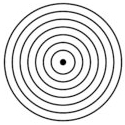
\includegraphics[]{pictures/doppler1.jpg}
    \caption{}
    \label{fig:doppler1}
\end{subfigure}
\begin{subfigure}{0.5\textwidth}
    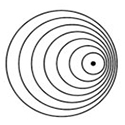
\includegraphics[]{pictures/doppler2.jpg}
    \caption{}
    \label{fig:doppler2}
\end{subfigure}

\end{figure}

Na obrazku \ref{fig:doppler1} źródło pozostaje w miejscu, natomiast na obrazku \ref{fig:doppler2} źródło \underline{porusza się}. Skutkiem tego ruchu jest zmiana długości fali i częstotliwości fali rejestrowanej przez obserwatora. Dla obserwatora znajdującego się z prawej strony źródła długość fali jest mniejsza, natomiast dla znajdującego się z lewej strony - wyższa.\\
 
Efekt Dopplera wyraża się wzorami:
\begin{table}[!h]
\centering
\begin{tabular}{|ll|}
\hline
\multicolumn{2}{|c|}{\textbf{Wzory}} \\ \hline
\multicolumn{1}{|l|}{Sytuacja 1} &  $f = f_0\frac{v}{v \pm v_z}$ \\ \hline
\multicolumn{1}{|l|}{Sytuacja 2} &  $f = f_0\frac{v \pm v_z}{v}$ \\ \hline
\multicolumn{1}{|l|}{Sytuacja 3} &  $f = f_0\frac{v\pm v_0}{v \pm v_z}$ \\ \hline
\end{tabular}
\caption{\textit{Wzory na efekt Dopplera}}\label{dopler}
\end{table}

gdzie:
\begin{itemize}
    \item [$\textbf{-}$]$f$ - częstotliwość rejestrowana przez obserwatora,
    \item [$\textbf{-}$]$f_0$ - częstotliwość źródła fali,
    \item [$\textbf{-}$]$v$ - prędkość fali,
    \item [$\textbf{-}$]$v_z$ - prędkość źródła,
    \item [$\textbf{-}$]$v_0$ - prędkość obserwatora.
\end{itemize}
\textwidth[1]{Przykłady}


Wzór \textbf{efektu Dopplera} przyjmuje 3 różne postaci (przedstawione w tabelce \ref{dopler}) w zależności od tego, kto się porusza - źródło czy obserwator. Możliwe są następujące sytuacje:


\begin{enumerate}
    \item Źródło porusza się, obserwator nie.
    \item Źródło nie porusza się, obserwator tak.
    \item Zarówno źródło jak i obserwator się poruszają.
\end{enumerate}

